\documentclass[10pt,twocolumn,letterpaper]{article}
\usepackage[utf8]{inputenc}
\usepackage{float}
\usepackage{hyperref}
\hypersetup{
    colorlinks=true,
    linkcolor=blue,
    filecolor=magenta,      
    urlcolor=cyan,
    pdftitle={Overleaf Example},
    pdfpagemode=FullScreen,
    }

% used for enhanced justification
\usepackage{microtype}

\usepackage[margin=0.6in]{geometry}

% used for indexing
\usepackage{index}
\makeindex

% used for images
\usepackage{graphics}
\graphicspath{ {./images/} }

% used for adjusting alignment for images
\usepackage[export]{adjustbox}

% used to stop images floating in strange ways
\usepackage[section]{placeins}

% used for nicer headers
\usepackage{fancyhdr}

% for the tables
\usepackage{multirow}
\usepackage{adjustbox}

% for pseudocode
\usepackage{listings}

% math packages
\usepackage{amssymb}
\usepackage{mathtools}
\usepackage{amsmath}
\usepackage{amsfonts}
\usepackage{amssymb}

\title{BitByteBeat: The Music Genre Classification Bot}
\author{Siu Ye, Johnny On, Chelsie Ng, Tyler Shanks}
\date{December 6 2021}

\begin{document}
\begin{titlepage}
   \begin{center}
       \vspace*{1cm}

       \Huge
       \textbf{BitByteBeat: The Music Genre Classification Bot}
       %\textbf{Machine Learning Course Project}

        \vspace{0.5cm}
        \Large
        Group 15: Siu Ye [40032209], Johnny On [40137434],\\
        Chelsie Ng [40071692], Tyler Shanks [401307528]
       
       \vspace{6cm}
        Machine Learning Course Project\\
        COMP 432\\
        Andrew Delong

        
       \vspace{1.5cm}
        
        \Large

       \vfill
            
       \vspace{0.8cm}
     
       
\includegraphics[width=0.4\textwidth]{images/concologo.png}

       Gina Cody School of Computer Science and Software Engineering\\
       Concordia University\\
       Canada\\
       December 6 2021
            
   \end{center}
\end{titlepage}


\fancyfoot{\thepage}

%\tableofcontents
%\addtocontents{toc}{\protect\enlargethispage{\baselineskip}}
%\newpage


% difference between \input and \include is that \include puts a \newpage after the 
% ref'd section is done
\section{Abstract}
    \paragraph{}
    We perform music genre classification manually using our own understanding of music. Methods that take into account conventional algorithmic approaches have not yet been developed since the distinctions between genres tend to be subjective and ill-defined. By observing and making predictions based on these ill-defined patterns, machine learning can observe and make predictions given enough audio data, of which large amounts can easily be harvested from online music. In this project, we aim to develop a music genre classifier that will accurately predict a song's genre by using a deep learning approach. Specifically, we will train two different models using two types of neural network architectures, namely, Convolution Neural Networks (CNN) and Recurrent Neural Networks (RNN). Python is used with a machine learning package: Tensorflow.keras to build our two models. We will compare and determine our best model through each of their accuracies.

\section{Introduction}
    \subsection{What are music genres?}
    \paragraph{}
    Music genres are essential tools for improving our understanding and enjoyment of music. A genre can be a powerful tool when searching for similar music or to highlight innovative musicians. As a tool for understanding and discussing artists' creations, genres are important because they are among the few and most valuable we have available. This way of categorizing sounds is flexible and descriptive, which can dramatically increase our ability to comprehend, recognize, and enjoy music. There are two ways to define a genre: the density of similar characteristics and the sparsity of distinctive features: dense clusters of productions form a music style, whereas pronounced differences define its edges \cite{kosina}. Nevertheless, there are gray areas in the classification of music genres that may cause overlap between categories \cite{iemtronics}. This is true whether reviewing a broad range of genres or an individual artist's discography.
    
    \subsection{Can we detect music genres?}
    \paragraph{}
    In spite of our varying levels of musical knowledge, it is very hard to explicitly define what a music genre a song belongs to just with our human ears \cite{iemtronics}. What makes jazz sound like jazz? And how can you tell the difference between hip hop and the blues? Computers or machines can use machine learning to build interpretive patterns based on data that is fed into them. Based on the data that is fed into the computer, machine learning can automatically create analytical models \cite{adragna_sun}. The power of machine learning principles comes into play when it comes to extracting music signatures from each genre \cite{guo_gu_liu}. We are then able to extract trends and patterns from a large dataset \cite{guo_gu_liu}. A number of techniques have been developed to help classify music genres based on how computers are used as new music equipment is being developed and deployed into our daily lives.
    
    \subsection{How to achieve our goal?}
    \paragraph{}
    Our main goal is to be able to make accurate predictions on a song’s genre. To achieve this, we will explore ways on how neural network architectures and splitting the training and testing data among groups affect our results and see if there are any benefits to do so. Python is used because there exists a collection and code stack of various open-source repositories and it is simple to understand \cite{python}. The Librosa Python module analyzes audio signals and is designed to be used for tracking music signals \cite{librosa}. It includes all of the parts to build a Music information retrieval (MIR) system. This module is very well documented and includes numerous examples and tutorials. Tensorflow is a Python-based scientific computing package. It is an open-source machine learning library used with the keras library designed to handle automatic differentiation libraries, which is helpful for implementing neural networks \cite{tensorflow}.
    
    \subsection{Which dataset will we use?}
    \paragraph{}
    The project’s data uses the GTZAN dataset \cite{kaggle} most frequently for evaluation. This dataset set includes a variety of recording-related sources (personal CDs, radio, microphone recordings), files were collected from 2000-2001. In particular, there are 10 genres, each with 100 audio files, all lasting 30 seconds each \cite{kaggle}. Using this dataset, we extract audio features, namely Mel-frequency Cepstral Coefficients (MFCC), from the raw data using the Librosa library. MFCCs are a small set of features that summarize the spectral envelope (often described in terms of timbre) \cite{haggblade_hong_kao}. They are frequently used in MIR. Since we cannot directly use the audio file as an input for our models, we need to preprocess it and then use the data in the GTZAN dataset. This means extracting useful features from the audio signal. Therefore, MFCC feature extraction is one of the ways to extract useful information from the signal because it defines the brightness of a sound \cite{haggblade_hong_kao}. It can also be used to calculate the timbre (quality) of the sound \cite{ceylan_hardala_kara_hardalac}. Then, a training set with category labels is provided for the purpose of training and evaluating the performances of the classifiers. A test set with no category labels is given to test the trained classifiers against unseen data.
 
    Everything will be and can be run from a Jupyter notebook. The initial step is to import all libraries needed for our project, regarding music genre classification. From the GTZAN dataset, we are able to load all songs in it. Once the dataset is loaded and saved via the dataset path, save\_mfcc is defined to perform the MFCCs extraction and save them into a .json file along with their respective genres. We divided each sample songs into different segments of 30 seconds and create our MFCCs. This ensures we have even more data to play around with. Once the data is ready and has been preprocessed, we can create both of our models for music genre classification.\\
    
    \subsection{Which models best suit our case?}
        \paragraph{}
        Convolution neural network is based on visual images. Its algorithms predict future datasets based on how they process and interpret visual images. CNN image classifications take an input image, process it and classify it under certain categories \cite{cnn_rnn}. Computers see an input image as an array of pixels and it depends on the image resolution. By analyzing images and recognizing information in images, machines can successfully analyze and classify future data \cite{cnn_rnn_2}. A CNN can classify music genres through the study of spectrograms (visual graphs of musical frequencies) which, in turn, enables machines to identify the category of particular types of music \cite{cnn_rnn}. Each input image passes through a series of convolution layers with kernels, pooling, fully connected layers and applies a softmax function to classify an object with probabilistic values between 0 and 1. 

        \paragraph{}
        Recurrent neural network learns how to remember sequences of information. Their unique characteristic is their memory, which draws on information from past inputs to influence current inputs and outputs \cite{cnn_rnn}. A pattern usually emerges when dealing with audio information from songs. These deep learning algorithms are commonly used for ordinal or temporal problems \cite{cnn_rnn_2}. As far as the RNN is concerned, it is a little different from traditional neural networks. It stores and uses the past data as information to predict future outcomes \cite{cnn_rnn}. The output from recurrent neural networks depends on the previous elements within the sequence, unlike traditional deep learning models which assume inputs and outputs are independent.
% \input{sections/intro-2}
\section{Methodologies}
    \subsection{Preprocessing}
        \paragraph{}
        An MFCC is a 2-D array. One dimension represents time while the other dimension represents the different frequencies. By analyzing the .json file created from the save\_mfcc method, we can observe the following. There are 9986 mfccs in total where each mfcc is mapped to a specific music genre. A genre is labelled as an integer from 0 to 9 because there are 10 different genres in our dataset (i.e. ['pop', 'metal', 'disco', 'blues', 'reggae', 'classical', 'rock', 'hiphop', 'country', 'jazz']). 
        
        Also, by looking at the distribution of our genres, we can see that it is evenly distributed. This is because the dataset contains 100 sample songs for each music genre. Note that, one song was removed in the jazz genre as jazz0054.wav was corrupted and could not be read. We can observed the genre distribution through our plot\_histogram function.
           \begin{figure}[H]
        \centering
        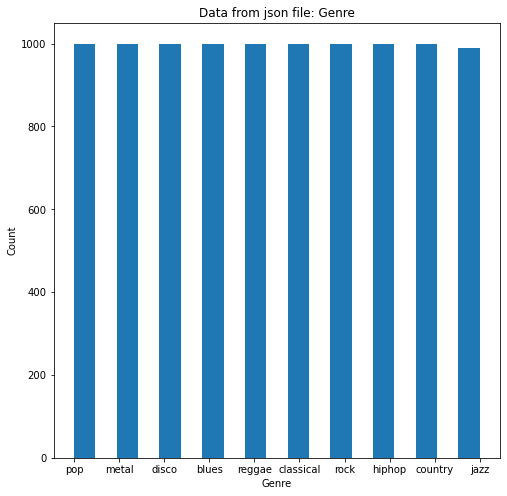
\includegraphics[width=0.35\textwidth]{images/genre.png} 
        \caption{Distribution of music genre data}
    \end{figure}
        
        \paragraph{}
        Also, the visual representation of each genre through a spectrogram which shows how quickly the frequencies themselves are changing over time. The first axis is frequency while the second axis is time. 
        
          \begin{figure}[H]
        \centering
        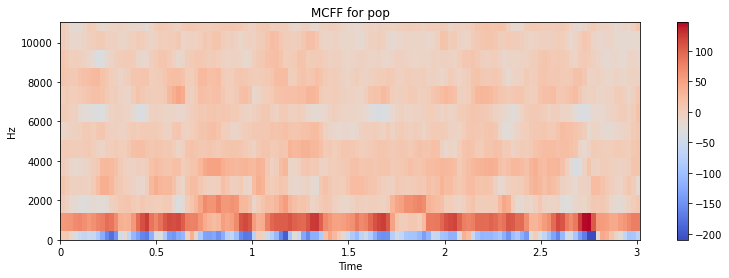
\includegraphics[width=0.5\textwidth]{images/pop_mfcc.png} 
        \caption{MFCC example}
        \end{figure}
        
    \subsection{Data Splitting}
        \paragraph{}    
        To have the data ready for training, we randomly split $(\boldsymbol{X}, \boldsymbol{y})$ into three parts, with no overlap. We separate $\boldsymbol{X}$ and $\boldsymbol{y}$ into 60\% training, 20\% validation and 20\% testing.
        
      
    \subsection{Training with CNN}
        \paragraph{}
        Our CNN model uses multiple layers. It is of sequential type. The input goes through these layers (specifically three convolution layers, one dense layer and one output layer) and at the end, the result gets flattened out and normalized into either one of ten possible results. Once the model has been created, the test data is fitted into it. When observing testing accuracy, we obtain the following result: 72.37\%
            
        \begin{figure}[H]
            \centering
            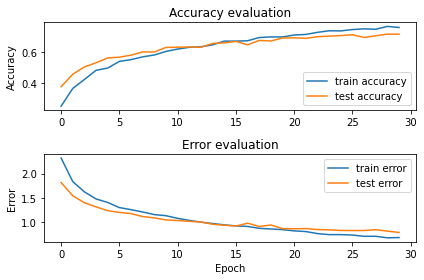
\includegraphics[width=0.45 \textwidth]{images/cnn_keras.png} 
            \caption{CNN accuracy/error evaluation}
        \end{figure}    
            
        \subsection{Training with RNN}
            \paragraph{}
            Our RNN model uses multiple layers as well. It is of sequential type. The input goes through these layers (two LSTM layers, one dense layer and one output layer). The result gets flattened out and normalized into either one of ten possible results of music genres. Once the model has been created, the test data is fitted into it. When observing testing accuracy, we obtain the following result: 59.11\%
            
        \begin{figure}[H]
            \centering
            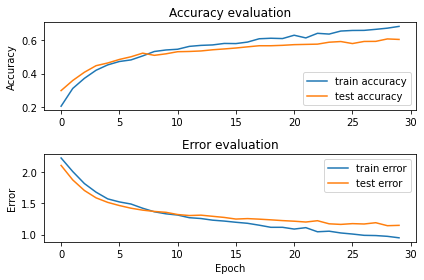
\includegraphics[width=0.45\textwidth]{images/rnn_keras.png} 
            \caption{RNN accuracy/error evaluation}
        \end{figure}
\section{Evaluation}
    \paragraph{}
    In this section, we will draw out conclusions from the models trained and compare them. As seen in section 3.3 and 3.4, we can conclude that our best model is CNN with 72.37\% accuracy.
    
    To further evaluate the models, we plotted their confusion matrix and classification report.
    
    \subsection{Confusion Matrix}
    \begin{figure}[H]
        \centering
        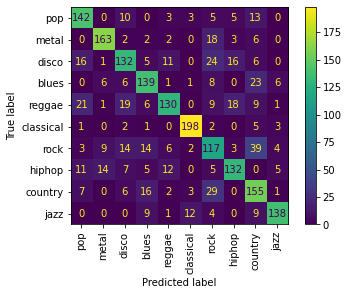
\includegraphics[width=0.35\textwidth]{images/cnn_matrix.png} 
        \caption{CNN confusion matrix}
    \end{figure}

    \begin{figure}[H]
        \centering
        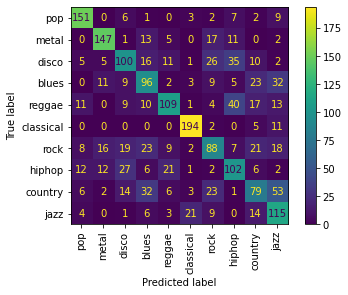
\includegraphics[width=0.35\textwidth]{images/rnn_matrix.png} 
        \caption{RNN confusion matrix}
    \end{figure}  
    
    \paragraph{}
    As we can see, from figure 5 and 6, the CNN made less errors than the RNN. Both has more accurately predicted classical music. Our CNN model misclassified rock as country the most while our RNN model misclassified country as jazz the most.
    
    From the diagonal of both confusion matrix, the CNN model performed way better.
    
    \subsection{Classification Report}
    \begin{figure}[H]
        \centering
        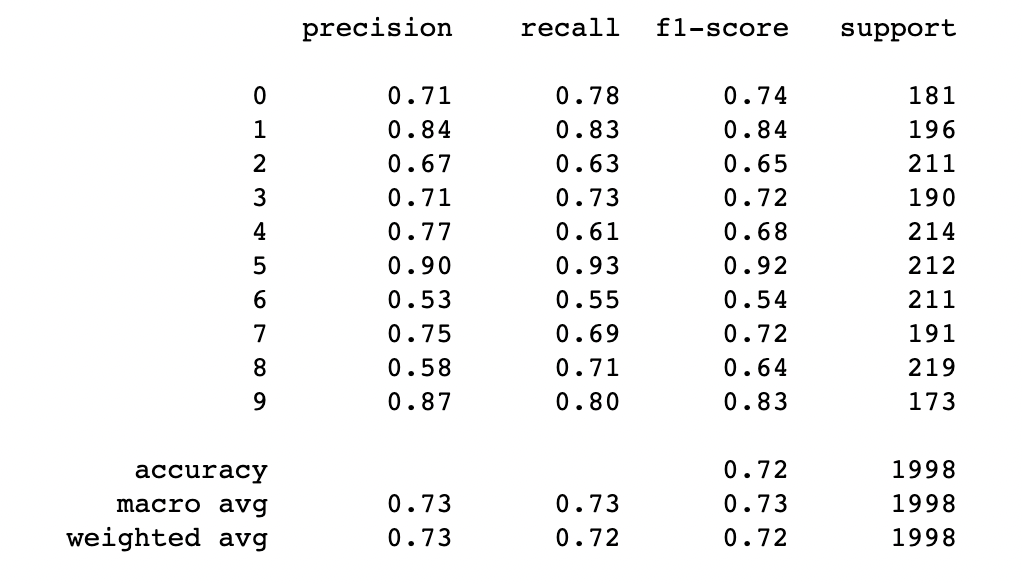
\includegraphics[width=0.4\textwidth]{images/cnn_classification_report.png} 
        \caption{CNN classification report}
    \end{figure}

    \begin{figure}[H]
        \centering
        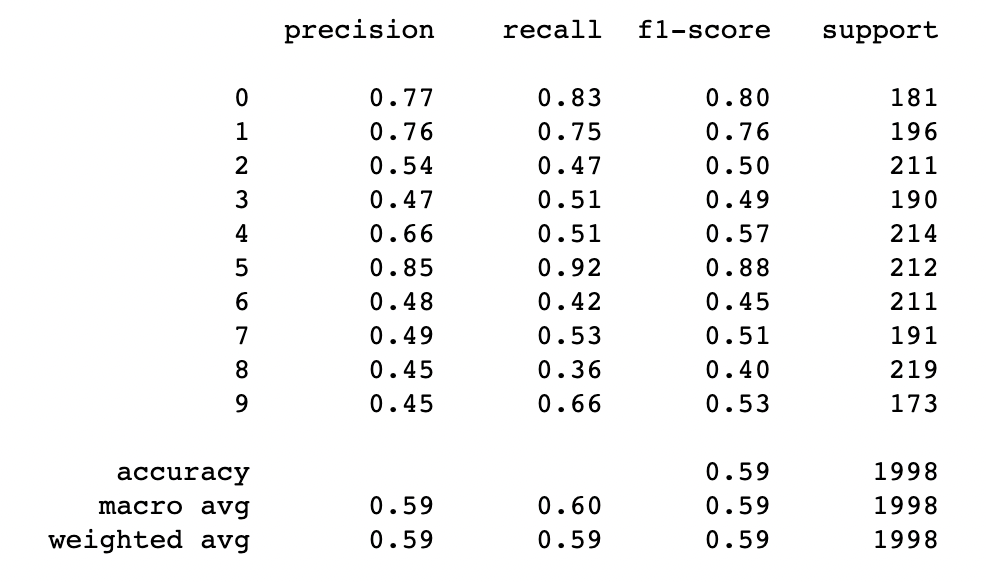
\includegraphics[width=0.4\textwidth]{images/rnn_classification_report.png} 
        \caption{RNN classification report}
    \end{figure}
    
    \paragraph{}
    Looking at the classification report from figure 7 and 8, our CNN model have higher precision, recall and f1-score. Our CNN model has on average 0.73 for all three metrics while our RNN model has 0.59, 0.60, 0.59 respectively.
    
    \paragraph{}
    To conclude, the CNN model had better precision and recall than the RNN model.
    
\section{Conclusion}
\paragraph{}
Finally, we are quite satisfied with the accuracies achieved. We were also able to create an interactive way for a user to use our model. The user would be able to copy and paste a YouTube link to the \href{https://github.com/xkaDachi/COMP432_Music_Classification/blob/main/Music%20Classification.ipynb}{jupyter notebook} itself and we would predict its genre with our best model (see figure 9).
\begin{figure}[H]
        \centering
        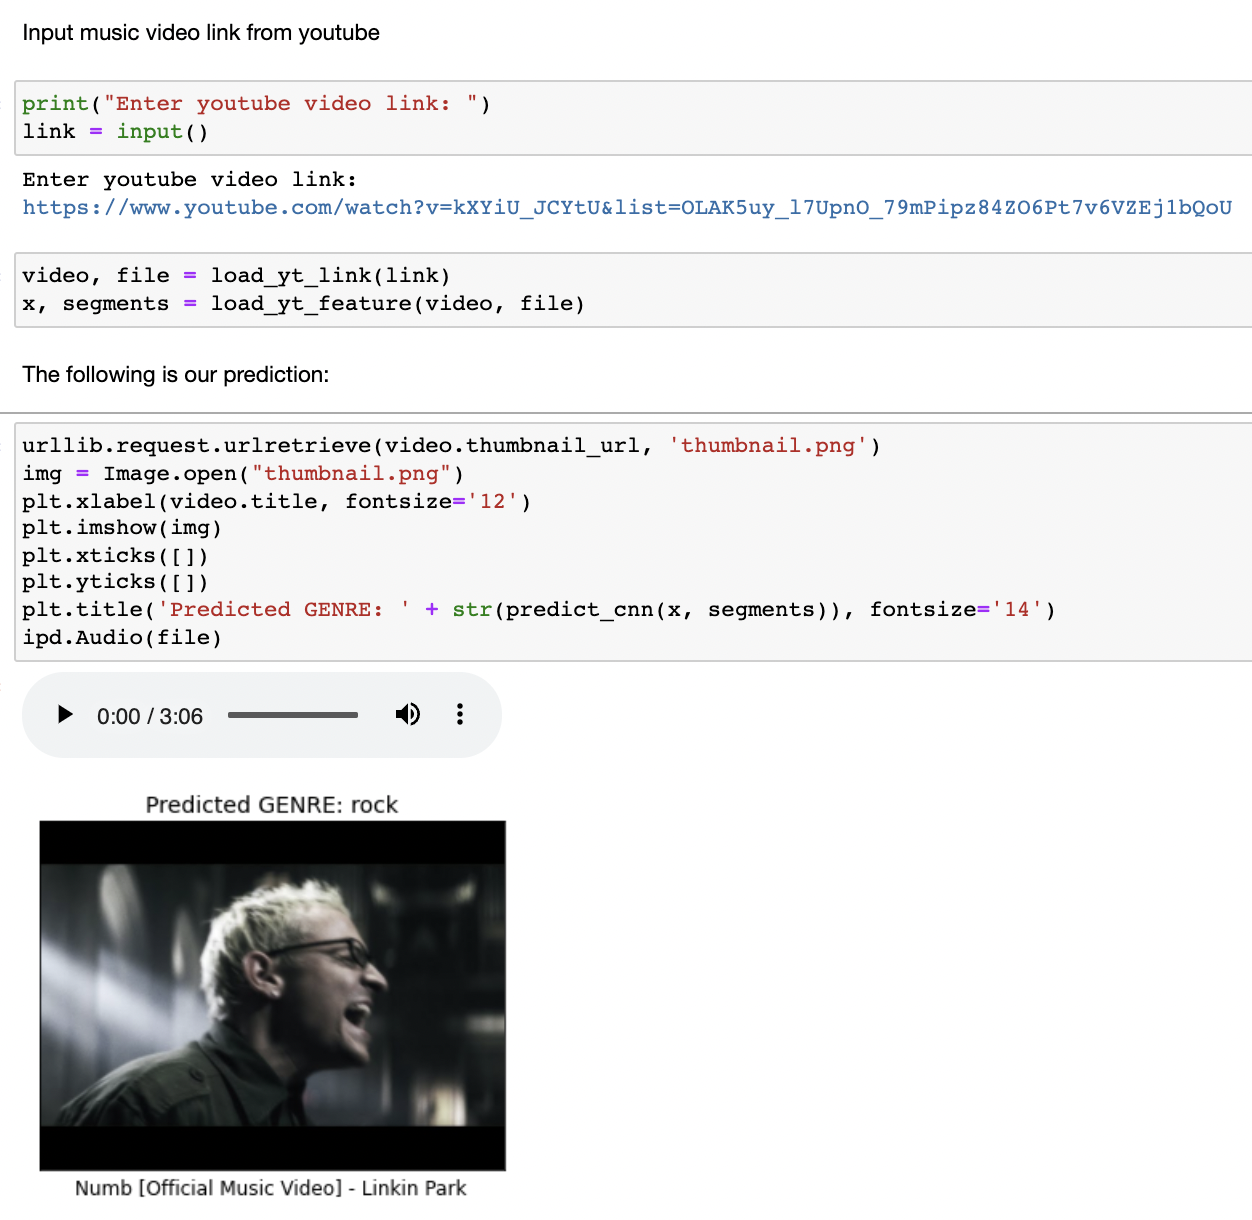
\includegraphics[width=0.4\textwidth]{images/yt_pred.png} 
        \caption{YouTube prediction}
    \end{figure}
\paragraph{}
In the event that we plan to further improve BitByteBeat, we agreed that we would require substantially more training data, both in the form of more genre types as well as overall dataset size. Genres change over time and our dataset currently has old songs. A major improvement would be to update our dataset with more recent songs. 
With this we could classify a larger set of songs more accurately.\\ 

In addition we also discussed the prospect of training it with other models like KNN or adding other audio features like volume, energy, pitch, etc along with the MFCC. We could also try applying feature selection techniques like Principal Component Analysis to identify optimal features to further improve results.\\

We have also looked into switching from the Keras framework of Tensorflow to the PyTorch framework. It could have been pleasant to compare the training speed of the model between the two frameworks and potentially see one of them being faster. It could have been interesting to analyze which model is better through its accuracy and testing between both CNN and RNN models depending on the framework used. \\

That being said, we can only talk about the 'what if' and 'why not' now because of all the knowledge we gained throughout the project. We indeed learned a lot and are very happy to have reached this level of completion. More specifically, it was really fun to try out our model on different YouTube songs and have a good laugh about it. It was a great introduction to Machine Learning for all of us!


% Bibliography here
% \newpage
\newpage
% \section{References}
\addcontentsline{toc}{section}{References}
\bibliographystyle{ieeetr}
\bibliography{sections/refs.bib}


\end{document}
